\documentclass[12pt]{report}
\usepackage{url}
\usepackage{amsmath}
\usepackage{xcolor}
\usepackage{listings}
\usepackage{graphicx}
\usepackage{parskip}
\usepackage{fancyhdr}
\usepackage{vmargin}
\usepackage{booktabs}
\usepackage{hyperref}
\usepackage[normalem]{ulem}
\usepackage{tabularray}
\usepackage{adjustbox}
\usepackage{lipsum}
\usepackage{caption}
\usepackage{subcaption}
\usepackage{cite}
\usepackage{cleveref}
\usepackage{textcomp}
\usepackage{multirow}
\usepackage{array}
\usepackage{amsmath}
\usepackage{mathtools}
\usepackage{amssymb}
\let\CheckCommand\providecommand
\usepackage{microtype}
\usepackage{stmaryrd}
\usepackage{float}
\usepackage{pdfpages}
\usepackage{diagbox}
\usepackage{tikz}
\usepackage{pgfplots}
\usepackage{pgfplotstable}
\usetikzlibrary{arrows, calc, positioning, tikzmark, automata, arrows.meta, decorations.markings}
\usepackage{titlesec}

% Numbers
\newcommand{\R}{\ensuremath{\mathbb{R}}}
\newcommand{\N}{\ensuremath{\mathbb{N}}}
\newcommand{\Z}{\ensuremath{\mathbb{Z}}}
\newcommand{\Q}{\ensuremath{\mathbb{Q}}}

% Fraktur
\newcommand{\A}{\ensuremath{\mathfrak A}}
\newcommand{\B}{\ensuremath{\mathfrak B}}
\newcommand{\I}{\ensuremath{\mathfrak I}}

% Logic
\newcommand{\xor}{\ensuremath{\oplus}}
\newcommand{\impl}{\ensuremath{\rightarrow}}

% Enumerations
\renewcommand{\labelenumi}{(\alph{enumi})}
\renewcommand{\labelenumii}{(\roman{enumii})}
\usepackage{enumitem}

\usepackage{bussproofs}
\newcommand{\yields}{\ensuremath{\mathrel{\Rightarrow}}}

\tikzset{
    graph node/.style = {draw, thick},
    labelled node/.style = {graph node, execute at begin node = {\strut}, execute at end node = {\strut}},
    round node/.style = {labelled node, shape = circle, inner sep = 1pt, minimum size = 9mm},
    rectangular node/.style = {labelled node, shape = rectangle, inner xsep = 5pt, inner ysep = 1pt, minimum size = 8mm},
    rounded node/.style = {labelled node, shape = rectangle, rounded corners = 4mm, inner ysep = 1pt, inner xsep = 5pt, minimum size = 9mm},
    player 0 node/.style = {round node, font = {\Large}},
    player 1 node/.style = {rectangular node, font = {\Large}},
    verifier node/.style = {rounded node, font = {\large}},
    falsifier node/.style = {rectangular node, font = {\large}},
    graph edge/.style = {draw, thick, shorten < = 2pt, shorten > = 2pt, > = {Latex[round, length = 2.5mm, width = 2.5mm]}},
    highlighted edge/.style = {graph edge, blue}
}

\lstset{
  language=Python,
  basicstyle=\ttfamily\small,
  keywordstyle=\color{blue}\bfseries,
  stringstyle=\color{red},
  commentstyle=\color{gray},
  showstringspaces=false,
  numbers=none,
  numberstyle=\tiny\color{gray},
  frame=single,
  breaklines=true,
}

\setmarginsrb{3 cm}{2.5 cm}{3 cm}{2.5 cm}{1 cm}{1.5 cm}{1 cm}{1.5 cm}

\title{Design and Implementation of a Data Warehouse for Product Engagement Analysis: A Case Study of Notion}
\author{Nick Zerjeski}
\date{November 2025}

\makeatletter
\let\thetitle\@title
\let\theauthor\@author
\let\thedate\@date
\makeatother

\pagestyle{fancy}
\fancyhf{}
\rhead{\theauthor}
\lhead{Data Warehouse for Product Engagement Analysis in Notion}
\cfoot{\thepage}

\begin{document}

% ------------------------------ TITLE PAGE ------------------------------
\begin{titlepage}
  \centering
  \vspace*{0.5 cm}
  
  \rule{\linewidth}{0.2 mm} \\[0.4 cm]
  {\huge \bfseries \thetitle}\\
  \rule{\linewidth}{0.2 mm} \\[1.5 cm]


  \begin{flushright}
    \large\theauthor\\
    \large\thedate
  \end{flushright}
\end{titlepage}

\tableofcontents
\newpage
\chapter{Domain Analysis and Description}\label{ch:1}
% Select a company and describe its domain
As the title suggests, in this case study we look at Notion. Notion is a Software-as-a-Service (SaaS) company that provides an all-in-one productivity and collaboration platform. It enables individuals and teams to create, organize, and share knowledge through a unified interface that combines note-taking, database management, task tracking, and wiki functionality. The platform is structured around \textit{workspaces} (multi-tenant units), which contain \textit{pages} composed of modular \textit{blocks} such as text, images, tables, and databases. These blocks are the atomic units of content and interaction. Workspaces can have multiple users, permission hierarchies, and integrations with external tools via API's.

% Describe the data landscape
The Notion ecosystem generates many voluminous data streams across several domains such as data about the Content, the User, Billing Data, Marketing and the Product Usage. In this case study we will focus on the Product Usage and Engagement. That is Event-level logs that captures user actions such as page creation, edits, views, comments, shares and API interactions. This data allows for temporal and behavioral analytics at high granularity.

% Data Warehouse Motivation (in this context)
A data warehouse is essential for Notion because its operational data is fragmented across multiple systems which are not optimized for analysis. Since the data is scattered it must be integrated into a consistent, subject-oriented repository to enable meaningful insights. A data warehouse provides stable, time-variant storage that preserves historical information necessary for analyzing trends in engagement and feature usage. This allows for fast, flexible querying of complex behavioral data. It also improves the data quality and consistency by cleaning and using heterogeneous sources. Therefore, a Data Warehouse enables us to transform raw event data into actionable intelligence. Ultimately, it provides the foundation for evidence-based decision-making and continuous product optimization.

\section{Key Analytical Questions}\label{sec:1.1}
The following five questions should later able to be answered by running queries on or data warehouse.

\begin{itemize}
\item \textbf{How does user engagement evolve over time across subscription tiers?}
This question reveals differences in activity between free and paid plans, supporting decisions on pricing and feature differentiation.

\item \textbf{Which content types (pages, databases, wikis, task boards) generate the highest sustained interaction rates?}  
Identifying the most engaging content structures helps prioritize feature development and template curation.

\item \textbf{What are the activation rates of new users within their first seven days?}  
Activation is a leading indicator of retention; understanding early engagement patterns enables targeted onboarding improvements.

\item \textbf{How does device usage (web, mobile, desktop) affect user activity and session duration?}  
Device-level analysis supports product optimization and informs cross-platform development priorities.

\item \textbf{What proportion of total activity originates from collaborative versus individual work?}  
Measuring the balance between solo and shared content usage reveals how effectively Notion fosters team adoption within workspaces.
\end{itemize}

\section{Key Performance Indicators (KPIs)}
Each analytical question corresponds to one or more measurable KPIs central to product health evaluation:

\begin{itemize}
\item \textbf{Daily/Weekly/Monthly Active Users (DAU/WAU/MAU):} Core activity metrics measuring recurring usage patterns.
\item \textbf{Stickiness Ratio (DAU/MAU):} Indicates habitual engagement and long-term adoption strength.
\item \textbf{Activation Rate:} Percentage of new users performing a predefined minimum number of meaningful interactions (e.g., seven content edits within seven days).
\item \textbf{Feature Adoption Rate:} Share of users engaging with advanced functionalities such as databases, templates, or integrations.
\item \textbf{Average Session Depth:} Mean number of interactions per user session, used to evaluate content richness and user intent.
\end{itemize}

\section{Granularity Discussion}
Since we are trying to analyze \textbf{Product Usage and Engagement} the appropriate granularity in this context are \textbf{Event-level facts}. Event-level facts capture each individual user action that occurs within a workspace, including page creations, edits, views, comments, shares, and API-driven interactions tied to a timestamp. Therefore, this level of detail is fine enough to compute all engagement-related KPIs. Furthermore, it ensures that every analytical question can be answered, since each fact retains its full context regarding each dimension. Using this level of granularity ensures analytical flexibility and avoids premature aggregation that would cause problems later one if a finer granularity would be required.


\chapter{Conceptual Design}
To build the Dimensional Fact Model, we first think about which dimensions and measures our fact should have. Since we are describing the Product Usage and Engagement our fact will represent a single atomic user event in Notion such as these described in Chapter \ref{ch:1}. To capture the full behavioral context, we need to capture also the user, the content object, the workspace, the device, the event type, the session and the timestamp, which we do via dimensions. We therefore have the following dimensions:
\begin{table}[H]
\centering
\begin{tabular}{ll}
\hline
\textbf{Attribute} & \textbf{Description} \\
\hline
\texttt{user\_id} & Unique identifier of the user \\
\texttt{signup\_date} & Date the user registered \\
\texttt{subscription\_tier} & Free, Plus, Business, Enterprise \\
\texttt{user\_type} & Individual, member, guest \\
\texttt{region} & User's geographic region \\
\texttt{lifecycle\_stage} & Onboarding, active, dormant, churn-risk \\
\hline
\end{tabular}
\caption{User Dimension}
\end{table}

\begin{table}[H]
\centering
\begin{tabular}{ll}
\hline
\textbf{Attribute} & \textbf{Description} \\
\hline
\texttt{content\_id} & Identifier of the page or block \\
\texttt{content\_type} & Page, database, wiki, task board, etc. \\
\texttt{is\_template\_based} & Indicates template-derived content \\
\texttt{is\_shared} & Whether content is shared with others \\
\texttt{ownership\_type} & Personal, workspace, or team space \\
\hline
\end{tabular}
\caption{Content Dimension}
\end{table}

\begin{table}[H]
\centering
\begin{tabular}{ll}
\hline
\textbf{Attribute} & \textbf{Description} \\
\hline
\texttt{workspace\_id} & Unique identifier of the workspace \\
\texttt{workspace\_plan} & Subscription plan of the workspace \\
\texttt{workspace\_size\_bucket} & Size category (1, 2--10, 11--50, 50+) \\
\texttt{industry\_segment} & Workspace industry classification \\
\texttt{workspace\_region} & Geographic region of workspace \\
\hline
\end{tabular}
\caption{Workspace Dimension}
\end{table}

\begin{table}[H]
\centering
\begin{tabular}{ll}
\hline
\textbf{Attribute} & \textbf{Description} \\
\hline
\texttt{device\_id} & Identifier for the device type \\
\texttt{platform} & Web, desktop, mobile \\
\texttt{operating\_system} & OS used for the event \\
\texttt{app\_version} & Client version \\
\texttt{device\_form\_factor} & Phone, tablet, desktop \\
\hline
\end{tabular}
\caption{Device Dimension}
\end{table}

\begin{table}[H]
\centering
\begin{tabular}{ll}
\hline
\textbf{Attribute} & \textbf{Description} \\
\hline
\texttt{event\_type} & View, edit, create, comment, share, etc. \\
\texttt{feature\_category} & Databases, templates, integrations, collaboration \\
\texttt{interaction\_intent} & Consumption, creation, collaboration \\
\hline
\end{tabular}
\caption{Event Dimension}
\end{table}

\begin{table}[H]
\centering
\begin{tabular}{ll}
\hline
\textbf{Attribute} & \textbf{Description} \\
\hline
\texttt{session\_id} & Unique session identifier \\
\texttt{session\_start\_time} & Start timestamp of the session \\
\texttt{session\_end\_time} & End timestamp of the session \\
\texttt{session\_origin} & Entry source (direct, link, notification) \\
\hline
\end{tabular}
\caption{Session Dimension}
\end{table}

\begin{table}[H]
\centering
\begin{tabular}{ll}
\hline
\textbf{Attribute} & \textbf{Description} \\
\hline
\texttt{date\_key} & Surrogate key for the date \\
\texttt{calendar\_date} & Full calendar date \\
\texttt{day\_of\_week} & Numeric day of week \\
\texttt{is\_weekend} & Weekend indicator \\
\texttt{week\_of\_year} & ISO week number \\
\texttt{month} & Month number \\
\texttt{quarter} & Calendar quarter \\
\texttt{year} & Calendar year \\
\texttt{day\_since\_signup\_bucket} & Bucket for activation/cohort logic \\
\hline
\end{tabular}
\caption{Time Dimension}
\end{table}
To evaluate product usage and engagement effectively, the fact table must also include measures that quantify how users interact with Notion. Therefore, the following measures allow us to aggregate individual events into meaningful indicators:

\textbf{Event Count}
\begin{itemize} % Important for possible aggregations later on
    \item \textbf{Description:} Always 1 per event.
    \item \textbf{Additivity:} Fully additive across all dimensions.
\end{itemize}

\textbf{Active User Flag}
\begin{itemize}
    \item \textbf{Description:} 1 on a user's first event of a day, 0 otherwise.
    \item \textbf{Additivity:} Additive across users for a fixed day; semi-additive across time.
\end{itemize}

\textbf{Activation Event Flag}
\begin{itemize}
    \item \textbf{Description:} 1 if the event is a meaningful interaction within the first seven days after signup.
    \item \textbf{Additivity:} Additive within user-time windows; non-additive when converted into activation rates.
\end{itemize}

\textbf{Feature Usage Flag}
\begin{itemize}
    \item \textbf{Description:} 1 if the event uses an advanced feature.
    \item \textbf{Additivity:} Additive for counts; non-additive when used in ratios.
\end{itemize}

\textbf{Collaboration Event Flag}
\begin{itemize}
    \item \textbf{Description:} 1 for events occurring in a collaborative context.
    \item \textbf{Additivity:} Additive for counts; non-additive for proportions.
\end{itemize}

\textbf{Session Event Count}
\begin{itemize}
    \item \textbf{Description:} Number of events per session (sum of Event Count grouped by session).
    \item \textbf{Additivity:} Additive within a session; semi-additive across time.
\end{itemize}

\textbf{Session Duration Seconds}
\begin{itemize}
    \item \textbf{Description:} Stored on the final event of a session.
    \item \textbf{Additivity:} Additive across sessions; semi-additive across time.
\end{itemize}


\section{Dimensional Fact Model}
Since we now discussed and defined the dimensions and measures of our Product Usage and Engagement fact, we can start building the Dimensional Fact Model (DFM).

\begin{figure}[ht]
\centering
\resizebox{\linewidth}{!}{%
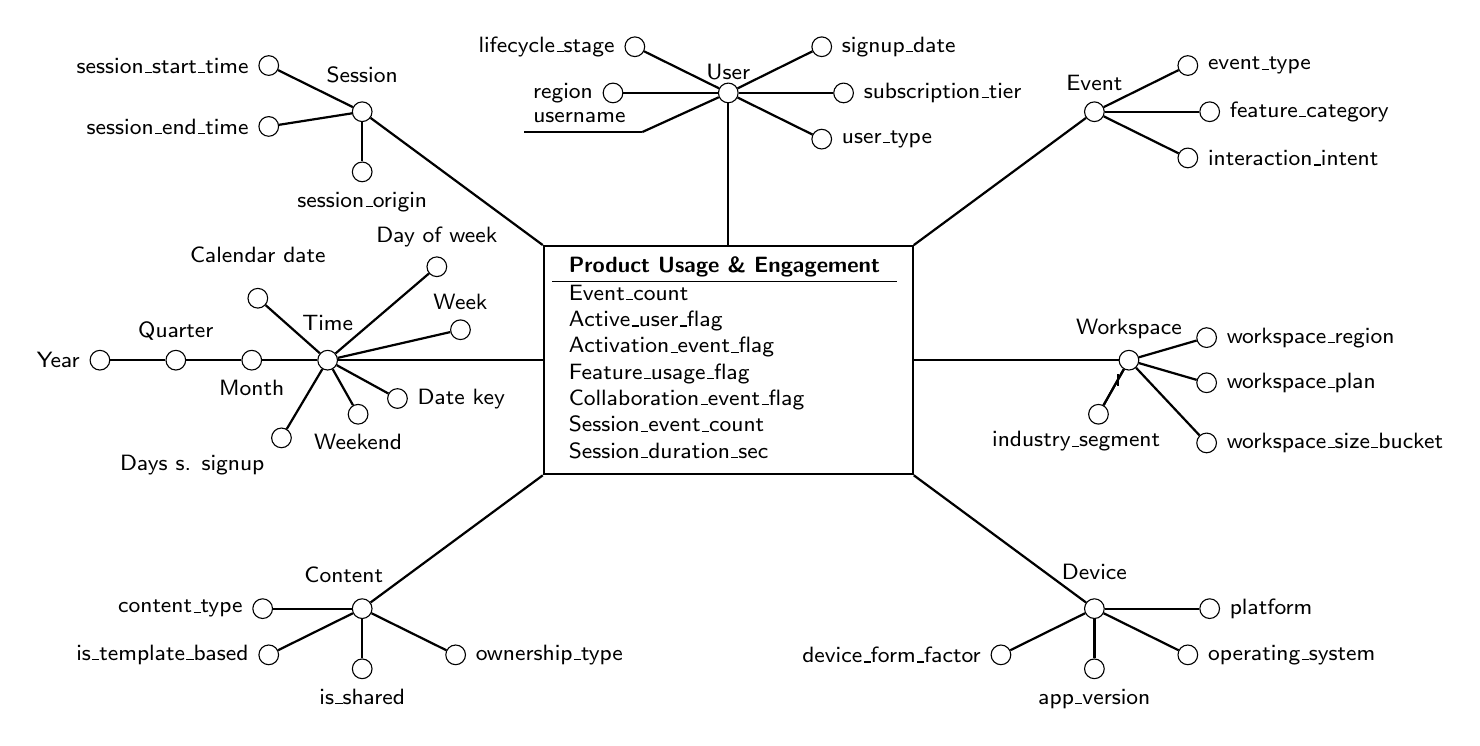
\begin{tikzpicture}[
  font=\sffamily\footnotesize,
  fact/.style={draw, rounded corners, thick, minimum width=40mm, minimum height=18mm, align=center},
  attr/.style={draw, circle, minimum size=2.5mm, inner sep=0pt},
  dimlbl/.style={fill=white, inner sep=1pt},
  >=latex
]

%==================== FACT ====================
\node[fact, draw, rounded corners=0, minimum width=0pt, inner sep=3pt] (F) {
    \begin{tabular}{l}
        \textbf{Product Usage \& Engagement} \\ \hline
        Event\_count \\
        Active\_user\_flag \\
        Activation\_event\_flag \\
        Feature\_usage\_flag \\
        Collaboration\_event\_flag \\
        Session\_event\_count \\
        Session\_duration\_sec \\
    \end{tabular}
};

%==================== TIME DIM ====================
\node[attr,left=26mm of F] (time0) {};
\node[dimlbl,above=2mm of time0] {Time};
\draw[-,thick] (time0) -- (F.west);

% Hierarchy: Date -> Week -> Month -> Quarter -> Year
\node[attr,left=7mm of time0] (timeMonth) {};
\node[below=0mm of timeMonth] {Month};
\node[attr,left=7mm of timeMonth] (timeQuarter) {};
\node[above=0mm of timeQuarter] {Quarter};
\node[attr,left=7mm of timeQuarter] (timeYear) {};
\node[left=0mm of timeYear] {Year};

\draw[thick] (timeYear) -- (timeQuarter) -- (timeMonth) -- (time0);

% Attributes attached to the Date level
\node[attr,above right=2mm and 15mm of time0] (timeDoW) {};
\node[above=0mm of timeDoW] {Week};
\draw[thick] (time0) -- (timeDoW);

\node[attr,above right=10mm and 12mm of time0] (week) {};
\node[above=0mm of week] {Day of week};
\draw[thick] (time0) -- (week);

\node[attr,below right=5mm and 2mm of time0] (timeWeekend) {};
\node[below=0mm of timeWeekend] {Weekend};
\draw[thick] (time0) -- (timeWeekend);

\node[attr,above left=6mm and 7mm of time0] (timeCalDate) {};
\node[above=2mm of timeCalDate] {Calendar date};
\draw[thick] (time0) -- (timeCalDate);

\node[attr,below left=8mm and 4mm of time0] (timeSignupBucket) {};
\node[below left=0mm of timeSignupBucket] {Days s. signup};
\draw[thick] (time0) -- (timeSignupBucket);

\node[attr,below right=3mm and 7mm of time0] (timeKey) {};
\node[right=0mm of timeKey] {Date key};
\draw[thick] (time0) -- (timeKey);

%==================== USER DIM ==================== USER name
\node[attr,above=18mm of F] (user0) {};
\node[dimlbl,above=0mm of user0] {User};
\draw[thick,-] (user0) -- (F.north);

% signup_date
\node[attr,above right=4mm and 10mm of user0] (userSignup) {};
\node[right=0mm of userSignup] {signup\_date};
\draw[thick] (user0) -- (userSignup);

% subscription_tier
\node[attr,right=12mm of user0] (userTier) {};
\node[right=0mm of userTier] {subscription\_tier};
\draw[thick] (user0) -- (userTier);

% user_type
\node[attr,below right=4mm and 10mm of user0] (userType) {};
\node[right=0mm of userType] {user\_type};
\draw[thick] (user0) -- (userType);

% username
\node[inner sep=0pt, minimum size=0pt, below left=4mm and 10mm of user0] (usernameHub) {};
\draw[thick] (user0) -- (usernameHub);

% left branch: username
\coordinate (usernameLeft) at ($(usernameHub)+(-15mm,0mm)$);
\draw[thick] ($(usernameHub)+(.1mm,0mm)$) -- (usernameLeft);
\node[above right=0mm and 0mm of usernameLeft] {username};


% region
\node[attr,left=12mm of user0] (userRegion) {};
\node[left=0mm of userRegion] {region};
\draw[thick] (user0) -- (userRegion);

% lifecycle_stage
\node[attr,above left=4mm and 10mm of user0] (userLife) {};
\node[left=0mm of userLife] {lifecycle\_stage};
\draw[thick] (user0) -- (userLife);


%==================== WORKSPACE DIM ====================
\node[attr,right=26mm of F] (ws0) {};
\node[dimlbl,above=1mm of ws0] {Workspace};
\draw[thick,-] (ws0) -- (F.east);

% subscription plan
\node[attr,below right=1mm and 8mm of ws0] (wsPlan) {};
\node[right=0mm of wsPlan] {workspace\_plan};
\draw[thick] (ws0) -- (wsPlan);

% size bucket
\node[attr,below=5mm of wsPlan] (wsSize) {};
\node[right=0mm of wsSize] {workspace\_size\_bucket};
\draw[thick] (ws0) -- (wsSize);

% industry segment (optional)
\node[attr,below left=5mm and 2mm of ws0] (wsInd) {};
\node[below left=0mm and -10mm of wsInd] {industry\_segment};
\draw[thick] (ws0) -- (wsInd);
% connection with optionality marker
\draw[thick] (ws0) -- (wsInd);
\path (ws0) -- (wsInd) coordinate[pos=0.3] (wsIndOpt);
\draw[thick] ($(wsIndOpt)+(0,-2.2pt)$) -- ($(wsIndOpt)+(0,2.2pt)$);

% geographic region
\node[attr,above right=1mm and 8mm of ws0] (wsRegion) {};
\node[right=0mm of wsRegion] {workspace\_region};
\draw[thick] (ws0) -- (wsRegion);

%==================== CONTENT DIM ==================== content name
\node[attr,below left=16mm and 22mm of F] (cont0) {};
\node[dimlbl,above left=2mm and -4mm of cont0] {Content};
\draw[thick,-] (cont0) -- (F.south west);

% content_type
\node[attr,left=10mm of cont0] (contType) {};
\node[left=0mm of contType] {content\_type};
\draw[thick] (cont0) -- (contType);

% is_template_based
\node[attr,below left=4mm and 10mm of cont0] (contTemplate) {};
\node[left=0mm of contTemplate] {is\_template\_based};
\draw[thick] (cont0) -- (contTemplate);

% is_shared
\node[attr,below=5mm of cont0] (contShared) {};
\node[below=0mm of contShared] {is\_shared};
\draw[thick] (cont0) -- (contShared);

% ownership_type
\node[attr,below right=4mm and 10mm of cont0] (contOwner) {};
\node[right=0mm of contOwner] {ownership\_type};
\draw[thick] (cont0) -- (contOwner);

%==================== DEVICE DIM ====================
\node[attr,below right=16mm and 22mm of F] (dev0) {};
\node[dimlbl,above=2mm of dev0] {Device};
\draw[thick,-] (dev0) -- (F.south east);

% platform
\node[attr,right=12mm of dev0] (devPlatform) {};
\node[right=0mm of devPlatform] {platform};
\draw[thick] (dev0) -- (devPlatform);

% operating_system
\node[attr,below right=4mm and 10mm of dev0] (devOS) {};
\node[right=0mm of devOS] {operating\_system};
\draw[thick] (dev0) -- (devOS);

% app_version
\node[attr,below=5mm of dev0] (devVersion) {};
\node[below=0mm of devVersion] {app\_version};
\draw[thick] (dev0) -- (devVersion);

% device_form_factor
\node[attr,below left=4mm and 10mm of dev0] (devForm) {};
\node[left=0mm of devForm] {device\_form\_factor};
\draw[thick] (dev0) -- (devForm);

%==================== EVENT DIM ====================
\node[attr,above right=16mm and 22mm of F] (evt0) {};
\node[dimlbl,above=1mm of evt0] {Event};
\draw[thick,-] (evt0) -- (F.north east);

% event_type
\node[attr,above right=4mm and 10mm of evt0] (evtType) {};
\node[right=0mm of evtType] {event\_type};
\draw[thick] (evt0) -- (evtType);

% feature_category
\node[attr,right=12mm of evt0] (evtFeat) {};
\node[right=0mm of evtFeat] {feature\_category};
\draw[thick] (evt0) -- (evtFeat);

% interaction_intent
\node[attr,below right=4mm and 10mm of evt0] (evtIntent) {};
\node[right=0mm of evtIntent] {interaction\_intent};
\draw[thick] (evt0) -- (evtIntent);


%==================== SESSION DIM ====================
\node[attr,above left=16mm and 22mm of F] (sess0) {};
\node[dimlbl,above=2mm of sess0] {Session};
\draw[thick,-] (sess0) -- (F.north west);

% session_start_time
\node[attr,above left=4mm and 10mm of sess0] (sessStart) {};
\node[left=0mm of sessStart] {session\_start\_time};
\draw[thick] (sess0) -- (sessStart);

% session_end_time
\node[attr,below left=0mm and 10mm of sess0] (sessEnd) {};
\node[left=0mm of sessEnd] {session\_end\_time};
\draw[thick] (sess0) -- (sessEnd);

% session_origin
\node[attr,below=5mm of sess0] (sessOrigin) {};
\node[below=0mm of sessOrigin] {session\_origin};
\draw[thick] (sess0) -- (sessOrigin);

\end{tikzpicture}
}
\caption{Dimensional Fact Model for Product Usage and Engagement.}
\end{figure}
TODO: Explaining the DFM and why I choose some of the design choices I made

\chapter{Logical Design}\label{ch:3}
Since all hierarchies are shallow and local to their dimensions and no hierarchy is reused across multiple dimensions, there is no need to normalize those hierarchies into additional tables. To keep the number of joins to a minimum and the queries as simple as possible, especially with no significant gain in storage efficiency, we are using a star schema for our \textit{Product Usage and Engagement} fact. Therefore, we have the following fact table, followed by the dimension tables.

\begin{table}[H]
\centering
\begin{tabular}{ll}
\hline
\textbf{Attribute} & \textbf{Key} \\
\hline
\texttt{usage\_id}            & Primary Key \\
\texttt{time\_key}           & FK$\rightarrow$ \texttt{dim\_time(time\_key)} \\
\texttt{user\_key}           & FK$\rightarrow$ \texttt{dim\_user(user\_key)} \\
\texttt{workspace\_key}      & FK$\rightarrow$ \texttt{dim\_workspace(workspace\_key)} \\
\texttt{content\_key}        & FK$\rightarrow$ \texttt{dim\_content(content\_key)} \\
\texttt{device\_key}         & FK$\rightarrow$ \texttt{dim\_device(device\_key)} \\
\texttt{event\_key}          & FK$\rightarrow$ \texttt{dim\_event(event\_key)} \\
\texttt{session\_key}        & FK$\rightarrow$ \texttt{dim\_session(session\_key)} \\
\texttt{event\_count}        &  \\
\texttt{active\_user\_flag}  &  \\
\texttt{activation\_event\_flag} &  \\
\texttt{feature\_usage\_flag}    &  \\
\texttt{collaboration\_event\_flag} &  \\
\texttt{session\_event\_count}    &  \\
\texttt{session\_duration\_sec}   &  \\
\hline
\end{tabular}
\caption{Fact table \texttt{fact\_product\_usage\_engagement}.}
\end{table}

\begin{table}[H]
\centering

\begin{minipage}{0.45\linewidth}
\centering
\begin{tabular}{l}
\hline
\textbf{Attribute} \\
\hline
\underline{\texttt{time\_key}} \\
\texttt{calendar\_date} \\
\texttt{day\_of\_week} \\
\texttt{is\_weekend} \\
\texttt{week\_of\_year} \\
\texttt{month} \\
\texttt{quarter} \\
\texttt{year} \\
\texttt{day\_since\_signup\_bucket} \\
\hline
\end{tabular}
\caption{Time table}
\end{minipage}
\hfill
\begin{minipage}{0.45\linewidth}
\centering
\begin{tabular}{l}
\hline
\textbf{Attribute} \\
\hline
\underline{\texttt{user\_key}} \\
\texttt{user\_id\_nat} \\
\texttt{signup\_date} \\
\texttt{subscription\_tier} \\
\texttt{user\_type} \\
\texttt{region} \\
\texttt{lifecycle\_stage} \\
\hline
\end{tabular}
\caption{User table}
\end{minipage}

\end{table}
\begin{table}[H]
\centering

\begin{minipage}{0.45\linewidth}
\centering
\begin{tabular}{l}
\hline
\textbf{Attribute} \\
\hline
\underline{\texttt{workspace\_key}} \\
\texttt{workspace\_id\_nat} \\
\texttt{workspace\_plan} \\
\texttt{workspace\_size\_bucket} \\
\texttt{industry\_segment} \\
\texttt{workspace\_region} \\
\hline
\end{tabular}
\caption{Workspace table}
\end{minipage}
\hfill
\begin{minipage}{0.45\linewidth}
\centering
\begin{tabular}{l}
\hline
\textbf{Attribute} \\
\hline
\underline{\texttt{content\_key}} \\
\texttt{content\_id\_nat} \\
\texttt{content\_type} \\
\texttt{is\_template\_based} \\
\texttt{is\_shared} \\
\texttt{ownership\_type} \\
\hline
\end{tabular}
\caption{Content table}
\end{minipage}

\end{table}
\begin{table}[H]
\centering

\begin{minipage}{0.45\linewidth}
\centering
\begin{tabular}{l}
\hline
\textbf{Attribute} \\
\hline
\underline{\texttt{device\_key}} \\
\texttt{device\_id\_nat} \\
\texttt{platform} \\
\texttt{operating\_system} \\
\texttt{app\_version} \\
\texttt{device\_form\_factor} \\
\hline
\end{tabular}
\caption{Device table}
\end{minipage}
\hfill
\begin{minipage}{0.45\linewidth}
\centering
\begin{tabular}{l}
\hline
\textbf{Attribute} \\
\hline
\underline{\texttt{event\_key}} \\
\texttt{event\_type} \\
\texttt{feature\_category} \\
\texttt{interaction\_intent} \\
\hline
\end{tabular}
\caption{Event table}
\end{minipage}

\end{table}
\begin{table}[H]
\centering
\begin{tabular}{l}
\hline
\textbf{Attribute} \\
\hline
\underline{\texttt{session\_key}} \\
\texttt{session\_id\_nat} \\
\texttt{session\_start\_time} \\
\texttt{session\_end\_time} \\
\texttt{session\_origin} \\
\hline
\end{tabular}
\caption{Session table}

\end{table}
To get an overview on how much space we will be using, we estimate the cardinality of our tables. For that, we assume that we save our data for two years. Furthermore, we assume that we have a user base of around five million users from which roughly \(20\%\) are active on a given day and produce around \(10\) interactions. Therefore, we have the following size of our fact table:
\[5\text{Mio User }\cdot 20\%\cdot10\text{ Interactions }\cdot730\text{ days}=7.3\cdot 10^9\text{ rows}\]
We further assume, that each workspace has on average ten users, which yields a total of \(500\)k rows for the workspace table. If each of the workspaces has around 50 content objects in it, the content table has \(25\)Mio rows. For the device dimension, we simply assume that there are \(100\) different devices available and we also have around 100 different types of events. Finally, for the session, we assume a day is a session. Therefore, we have 
\[5\text{Mio User }\cdot 20\%\cdot730\text{ days}=7.3\cdot 10^8\text{ rows}\]
for the session table. To simplify the calculation of the size of the table, we assume that each column takes \(8\) Bytes. With that our tables have the sizes specified in Table \ref{tab:siz}. Keep in mind that some values are rounded.
\begin{table}[H]
\centering
\begin{tabular}{lr}
\hline
\textbf{Table} & \textbf{Size}\\
\hline
\text{Product Usage Engagement}  & 800GB \\
\text{Session}  & 30GB \\
\text{Content}  & 1GB \\
\text{User}  & 26MB \\
\text{Workspace}  & 23MB \\
\text{Time}  & 50KB \\
\text{Device}  & 5KB \\
\text{Event}  & 3KB \\
\hline
\end{tabular}
\caption{Sizes of the tables.}\label{tab:siz}
\end{table}


\section{Demonstration}
Now that we have the logical model in place, it is ready to support analytical workflows. To demonstrate how our schema answers to the defined business questions in section \ref{sec:1.1}, we select two of them and express them directly in SQL to extract the data from our  newly created fact and dimension tables. To be able to do this, we first have to populate our tables with some mock data. Note that only attributes are specified, that are needed for the analytical query.

\begin{table}[H]
\centering
\begin{tabular}{ccccc}
\hline
\textbf{usage\_id} & \textbf{time\_key} & \textbf{user\_key} & \textbf{content\_key} & \textbf{event\_count} \\
\hline
1  & 1 & 10 & 100 & 1 \\
2  & 1 & 10 & 100 & 1 \\
3  & 1 & 11 & 101 & 1 \\
4  & 1 & 12 & 102 & 1 \\
5  & 2 & 10 & 100 & 1 \\
6  & 2 & 11 & 101 & 1 \\
7  & 2 & 12 & 101 & 1 \\
8  & 3 & 10 & 100 & 1 \\
9  & 3 & 11 & 102 & 1 \\
10 & 3 & 12 & 100 & 1 \\
\hline
\end{tabular}
\caption{Mock data for \texttt{fact\_product\_usage\_engagement}.}
\end{table}

\begin{table}[H]
\centering

\begin{minipage}{0.45\linewidth}
\centering
\begin{tabular}{cc}
\hline
\textbf{time\_key} & \textbf{calendar\_date} \\
\hline
1 & 2025-01-01 \\
2 & 2025-01-02 \\
3 & 2025-01-03 \\
\hline
\end{tabular}
\caption{Mock data for \texttt{dim\_time}.}
\end{minipage}
\hfill
\begin{minipage}{0.45\linewidth}
\centering
\begin{tabular}{cc}
\hline
\textbf{user\_key} & \textbf{subscription\_tier} \\
\hline
10 & Free \\
11 & Plus \\
12 & Free \\
\hline
\end{tabular}
\caption{Mock data for \texttt{dim\_user}.}
\end{minipage}

\end{table}

\begin{table}[H]
\centering
\begin{tabular}{cc}
\hline
\textbf{content\_key} & \textbf{content\_type} \\
\hline
100 & page \\
101 & database \\
102 & wiki \\
\hline
\end{tabular}
\caption{Mock data for \texttt{dim\_content}.}
\end{table}

With the mock data in place, we can go to our business questions. As first question we choose
\begin{quote}
    How does user engagement evolve over time across subscription tiers?
\end{quote}
This is an important question for subscription-based SaaS products, since different user tiers often exhibit different engagement patterns. Understanding how frequently users in each tier interact with the platform over time allows to identify trends in adoption, retention, and value perception. In Listing \ref{lst:bq1} you can see the query that extracts the information needed for answering this question.
\begin{lstlisting}[language=SQL,caption={Query for answering: How does user engagement evolve over time across subsciption tiers?},label={lst:bq1},captionpos=b]
SELECT
    t.calendar_date,
    u.subscription_tier,
    SUM(f.event_count) AS total_events
FROM fact_product_usage_engagement AS f
JOIN dim_time AS t
    ON f.time_key = t.time_key
JOIN dim_user AS u
    ON f.user_key = u.user_key
GROUP BY
    t.calendar_date,
    u.subscription_tier
ORDER BY
    t.calendar_date,
    u.subscription_tier;
\end{lstlisting}
The result of running this query can be seen in Table \ref{tbl:bq1-results}.
\begin{table}[H]
\centering
\begin{tabular}{lcc}
\hline
\textbf{calendar\_date} & \textbf{subscription\_tier} & \textbf{total\_events} \\
\hline
2025-01-01 & Free & 3 \\
2025-01-01 & Plus & 1 \\
2025-01-02 & Free & 2 \\
2025-01-02 & Plus & 1 \\
2025-01-03 & Free & 2 \\
2025-01-03 & Plus & 1 \\
\hline
\end{tabular}
\caption{Resulting table after running the query in Listing \ref{lst:bq1}.}\label{tbl:bq1-results}
\end{table}

The second business question for which we run the query on is
\begin{quote}
    Which content types generate the highest interaction rates?
\end{quote}
This is an important business question because different content types are related to different workflows, and their usage patterns are strong indicators of feature adoption. Analyzing it provides insights on how future features can be developed. In Listing \ref{lst:bq2} you can see the query that extracts the information needed for answering this question.
\begin{lstlisting}[language=SQL,caption={Query for answering: Which content types generate the highest interaction rates?},label={lst:bq2},captionpos=b]
SELECT
    c.content_type,
    SUM(f.event_count) AS total_events
FROM fact_product_usage_engagement AS f
JOIN dim_content AS c
    ON f.content_key = c.content_key
GROUP BY
    c.content_type
ORDER BY
    total_events DESC;
\end{lstlisting}
The result of this query can be seen in Table \ref{tbl:bq2-results}.
\begin{table}[H]
\centering
\begin{tabular}{lc}
\hline
\textbf{content\_type} & \textbf{total\_events} \\
\hline
page     & 5 \\
database & 3 \\
wiki     & 2 \\
\hline
\end{tabular}
\caption{Resulting table after running the query in Listing \ref{lst:bq2}.}\label{tbl:bq2-results}
\end{table}
\chapter{Physical Design}
Now that the logical design is in place, we can start to implement it in a real database system. For that, we create a script that creates all the tables with their corresponding surrogate keys and relations we defined in Chapter \ref{ch:3}. A snippet of this script can be seen in Listing \ref{lst:cs1}. Keep in mind that the full scripts are provided as appendix.
\begin{lstlisting}[language=SQL,caption={Snippet of the script for creating the Data Warehouse.},label={lst:cs1},captionpos=b]
-- Creation of the user dimension
CREATE TABLE IF NOT EXISTS dim_user (
  user_key    INT GENERATED ALWAYS AS IDENTITY PRIMARY KEY,
  user_id_nat VARCHAR(64) NOT NULL UNIQUE,
  signup_date DATE,
  ...
);

-- Snippet of the fact table
CREATE TABLE IF NOT EXISTS fact_product_usage_engagement (
  usage_id    BIGINT GENERATED ALWAYS AS IDENTITY,
  time_key    INT NOT NULL,
  ...
  PRIMARY KEY (usage_id, time_key),
  CONSTRAINT fk_fact_user
        FOREIGN KEY (user_key) REFERENCES dim_user(user_key),
) PARTITION BY RANGE (time_key);
\end{lstlisting}
Here we can see that every attribute with a \_key postfix is a surrogate key. As you can see in Table \ref{tab:siz}, the fact table can get rather big. It is therefore useful to split it into smaller tables. For our Key Analytical Questions we want to answer later on, it is beneficial to partition the table on the time dimension.

To populate our data warehouse, we first have to define in which time span we want to have data in it. Since data warehouses normally store data for up to two years, we choose January 2024 to December 2025 as the time span in which we want to store data in it. Of course, we can not simply add random data to it, because then we couldn't get meaningful data to answer our analytical questions. Therefore, we did the following assumptions: 


First, we created monthly partitions for the fact table so that the data fits into the chosen time span and queries stay fast. Then we filled the time dimension with one row per day from 2024-01-01 to 2025-12-31 so that every event can be linked to a calendar day. We also set up small, fixed device, content, and event dimensions with realistic options - for example desktop vs. mobile, wiki vs. or database vs. page - to make sure we have meaningful categories instead of random strings.

For the user dimension, we generated 20 new users per month across the whole time span, which yields 480 total users. We varied subscription tier, user type, region, and life cycle stage in a deterministic way so each month is stable in that regard and we can compare Free vs. Plus vs. Business vs. Enterprise behavior. Workspaces were created separately with at least 50 entries that mix plans, size buckets, industries, and regions to keep workspaces varied without being chaotic.

Sessions were added at about five per day, with durations between roughly 20 and 70 minutes. This gives enough session coverage so that every event can find a plausible session on the same day.

Finally, the fact table generation ties everything together. We compute an activation probability per user based on their tier and only give activation events to users who pass that threshold in their first week. On top of that, we assign monthly event volumes per user that scale with their tier, then sprinkled some randomness in it to avoid overly uniform behavior.

For each event we pick a date within the valid window, that is an event can only occur after a user created their account, attach biased mixes for content types, devices, and event types, and link the event to a workspace and a same-day session. The measure flags are set according to the type of event and content so that activation, feature usage, and collaboration metrics come out believable. This way the warehouse ends up with structured, meaningful mock data so we are ready to answer our key analytical questions. All scripts that answers those questions are provided in the appendix.

For our first question, we wanted to know how the user engagement evolves over multiple tiers.
\end{document}